\subsection{Zone d'étude}

Notre analyse s'est concentrée sur les données collectées du banc Swiftsure, à l'ouest du détroit de Juan de Fuca, vers l'est jusqu'aux îles Gulf et San Juan dans le sud de la mer des Salish (Figure \ref{fig:study-area}). Nous avons contraint notre analyse à cette région basée sur la disponibilité des données de régime alimentaire de l'ÉRES et les estimations publiées précédemment de l'utilisation de l'habitat des ÉRE \citep{thorntonSouthernResidentKiller2022}. Bien que les ÉRES se trouvent au sud jusqu'en Californie centrale et au nord jusqu'au centre de la Colombie-Britannique, notre zone d'étude comprend l'habitat essentiel que la population utilise extensivement de mai à novembre \citep{dfoIdentificationHabitatsSpecial2017}. Dans le domaine d'étude, nous avons défini des strates spatiales pour visualiser les échantillons de régime alimentaire de l'ÉRES et dépendants de la pêcherie, ainsi que pour générer des prédictions saisonnières spatialement-explicites (Figure \ref{fig:sampling-map}) ; cependant, ces strates n'ont pas été incorporées comme paramètres de modèle, qui ont incorporé les données spatiales, c.-à-d. les coordonnées, directement (détails additionnels ci-dessous).

\begin{figure}[H]
    \centering
    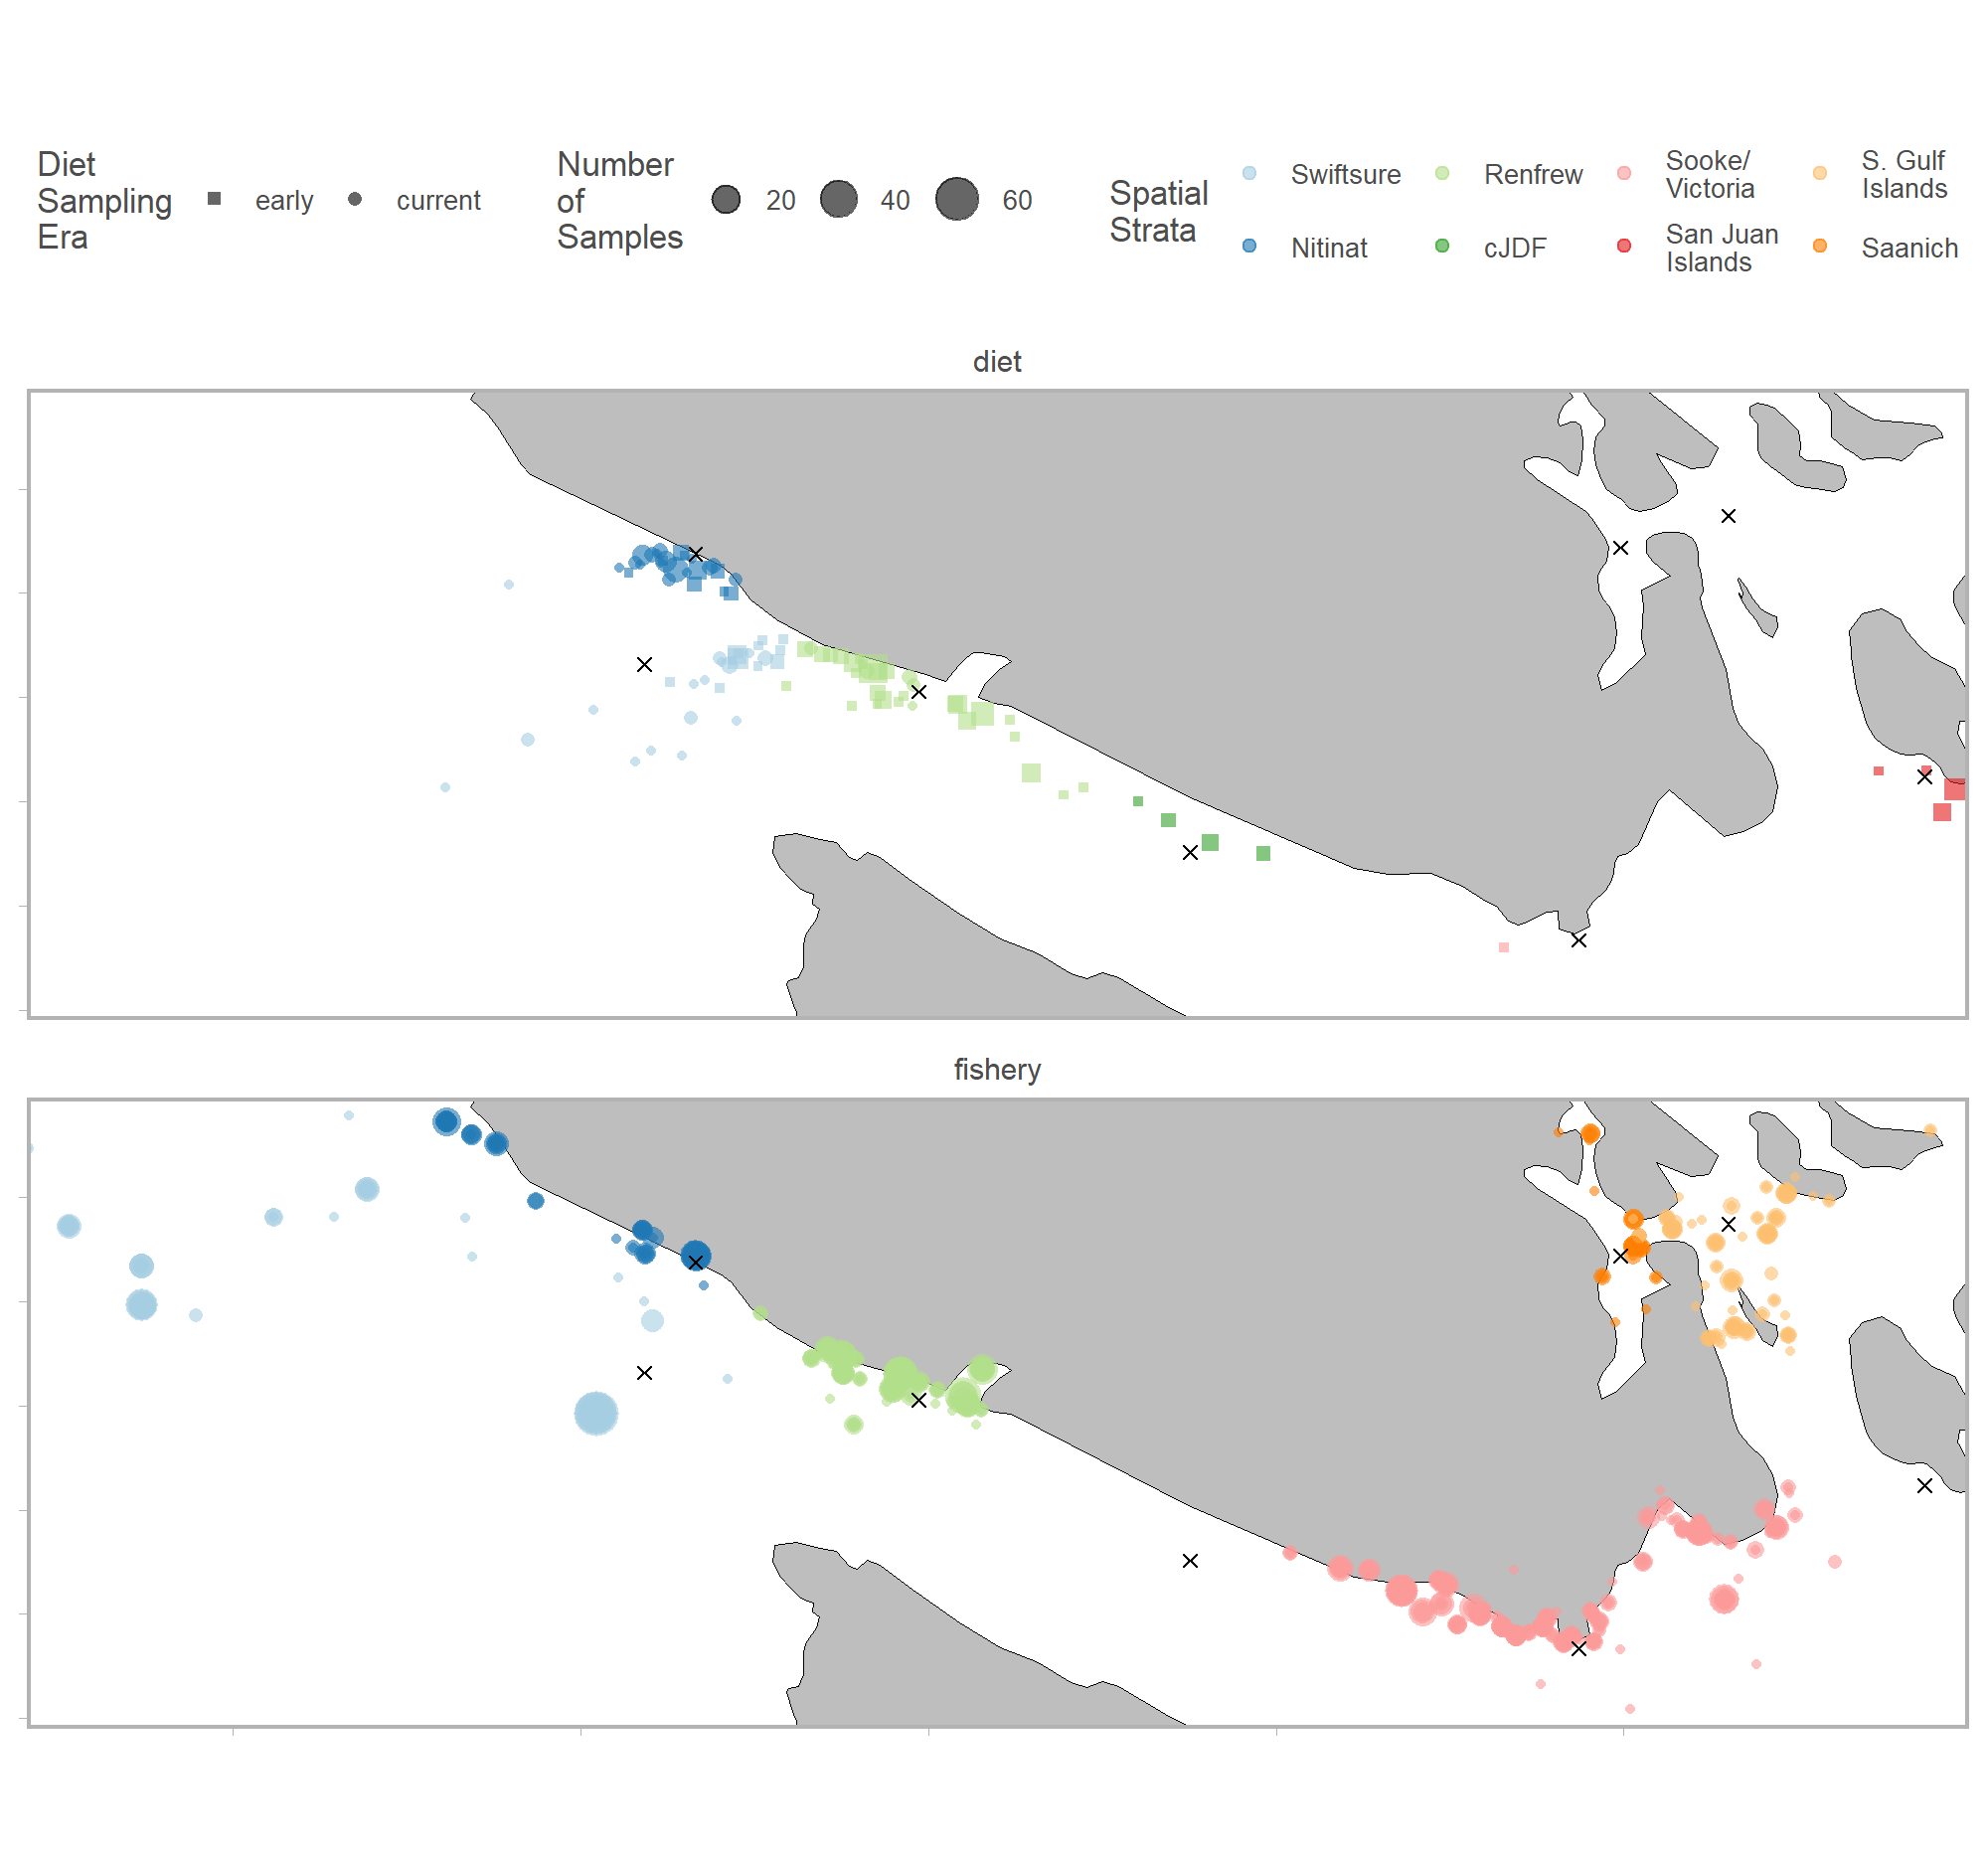
\includegraphics[width=5in]{figs/study_area.png}
    \caption{Zone d'étude dans le sud côtier de la Colombie-Britannique. La bathymétrie du fond marin représentée par l'ombrage bleu et l'habitat essentiel de l'ÉRES dénoté par le polygone ombragé gris.}
    \label{fig:study-area}
\end{figure}

\subsection{Échantillonnage des restes de proies de l'ÉRES}

La collecte des restes de proies d'épaulard résident a commencé en 1974 dans le cadre de l'étude à long terme du MPO sur l'histoire de vie des épaulards. De 2003 à 2013 (désignée comme « période d'échantillonnage précoce »), des relevés côtiers dédiés sur l'alimentation des ÉRE ont été entrepris principalement en utilisant un navire à moteur de 10 m \citep{fordChinookSalmonPredation2010, fordLinkingKillerWhale2010}. Les échantillons obtenus de 2017 à 2023 sont référés comme la « période d'échantillonnage actuelle » et ont été collectés principalement de relevés près du banc Swiftsure en utilisant des embarcations pneumatiques à coque rigide de 7 m \citep{thorntonSouthernResidentKiller2022}, avec trois années d'effort de relevé (2018-2020) s'étendant le long du détroit de Juan de Fuca jusqu'à Sooke (Figure \ref{fig:sampling-map}).

\begin{figure}[H]
    \centering
    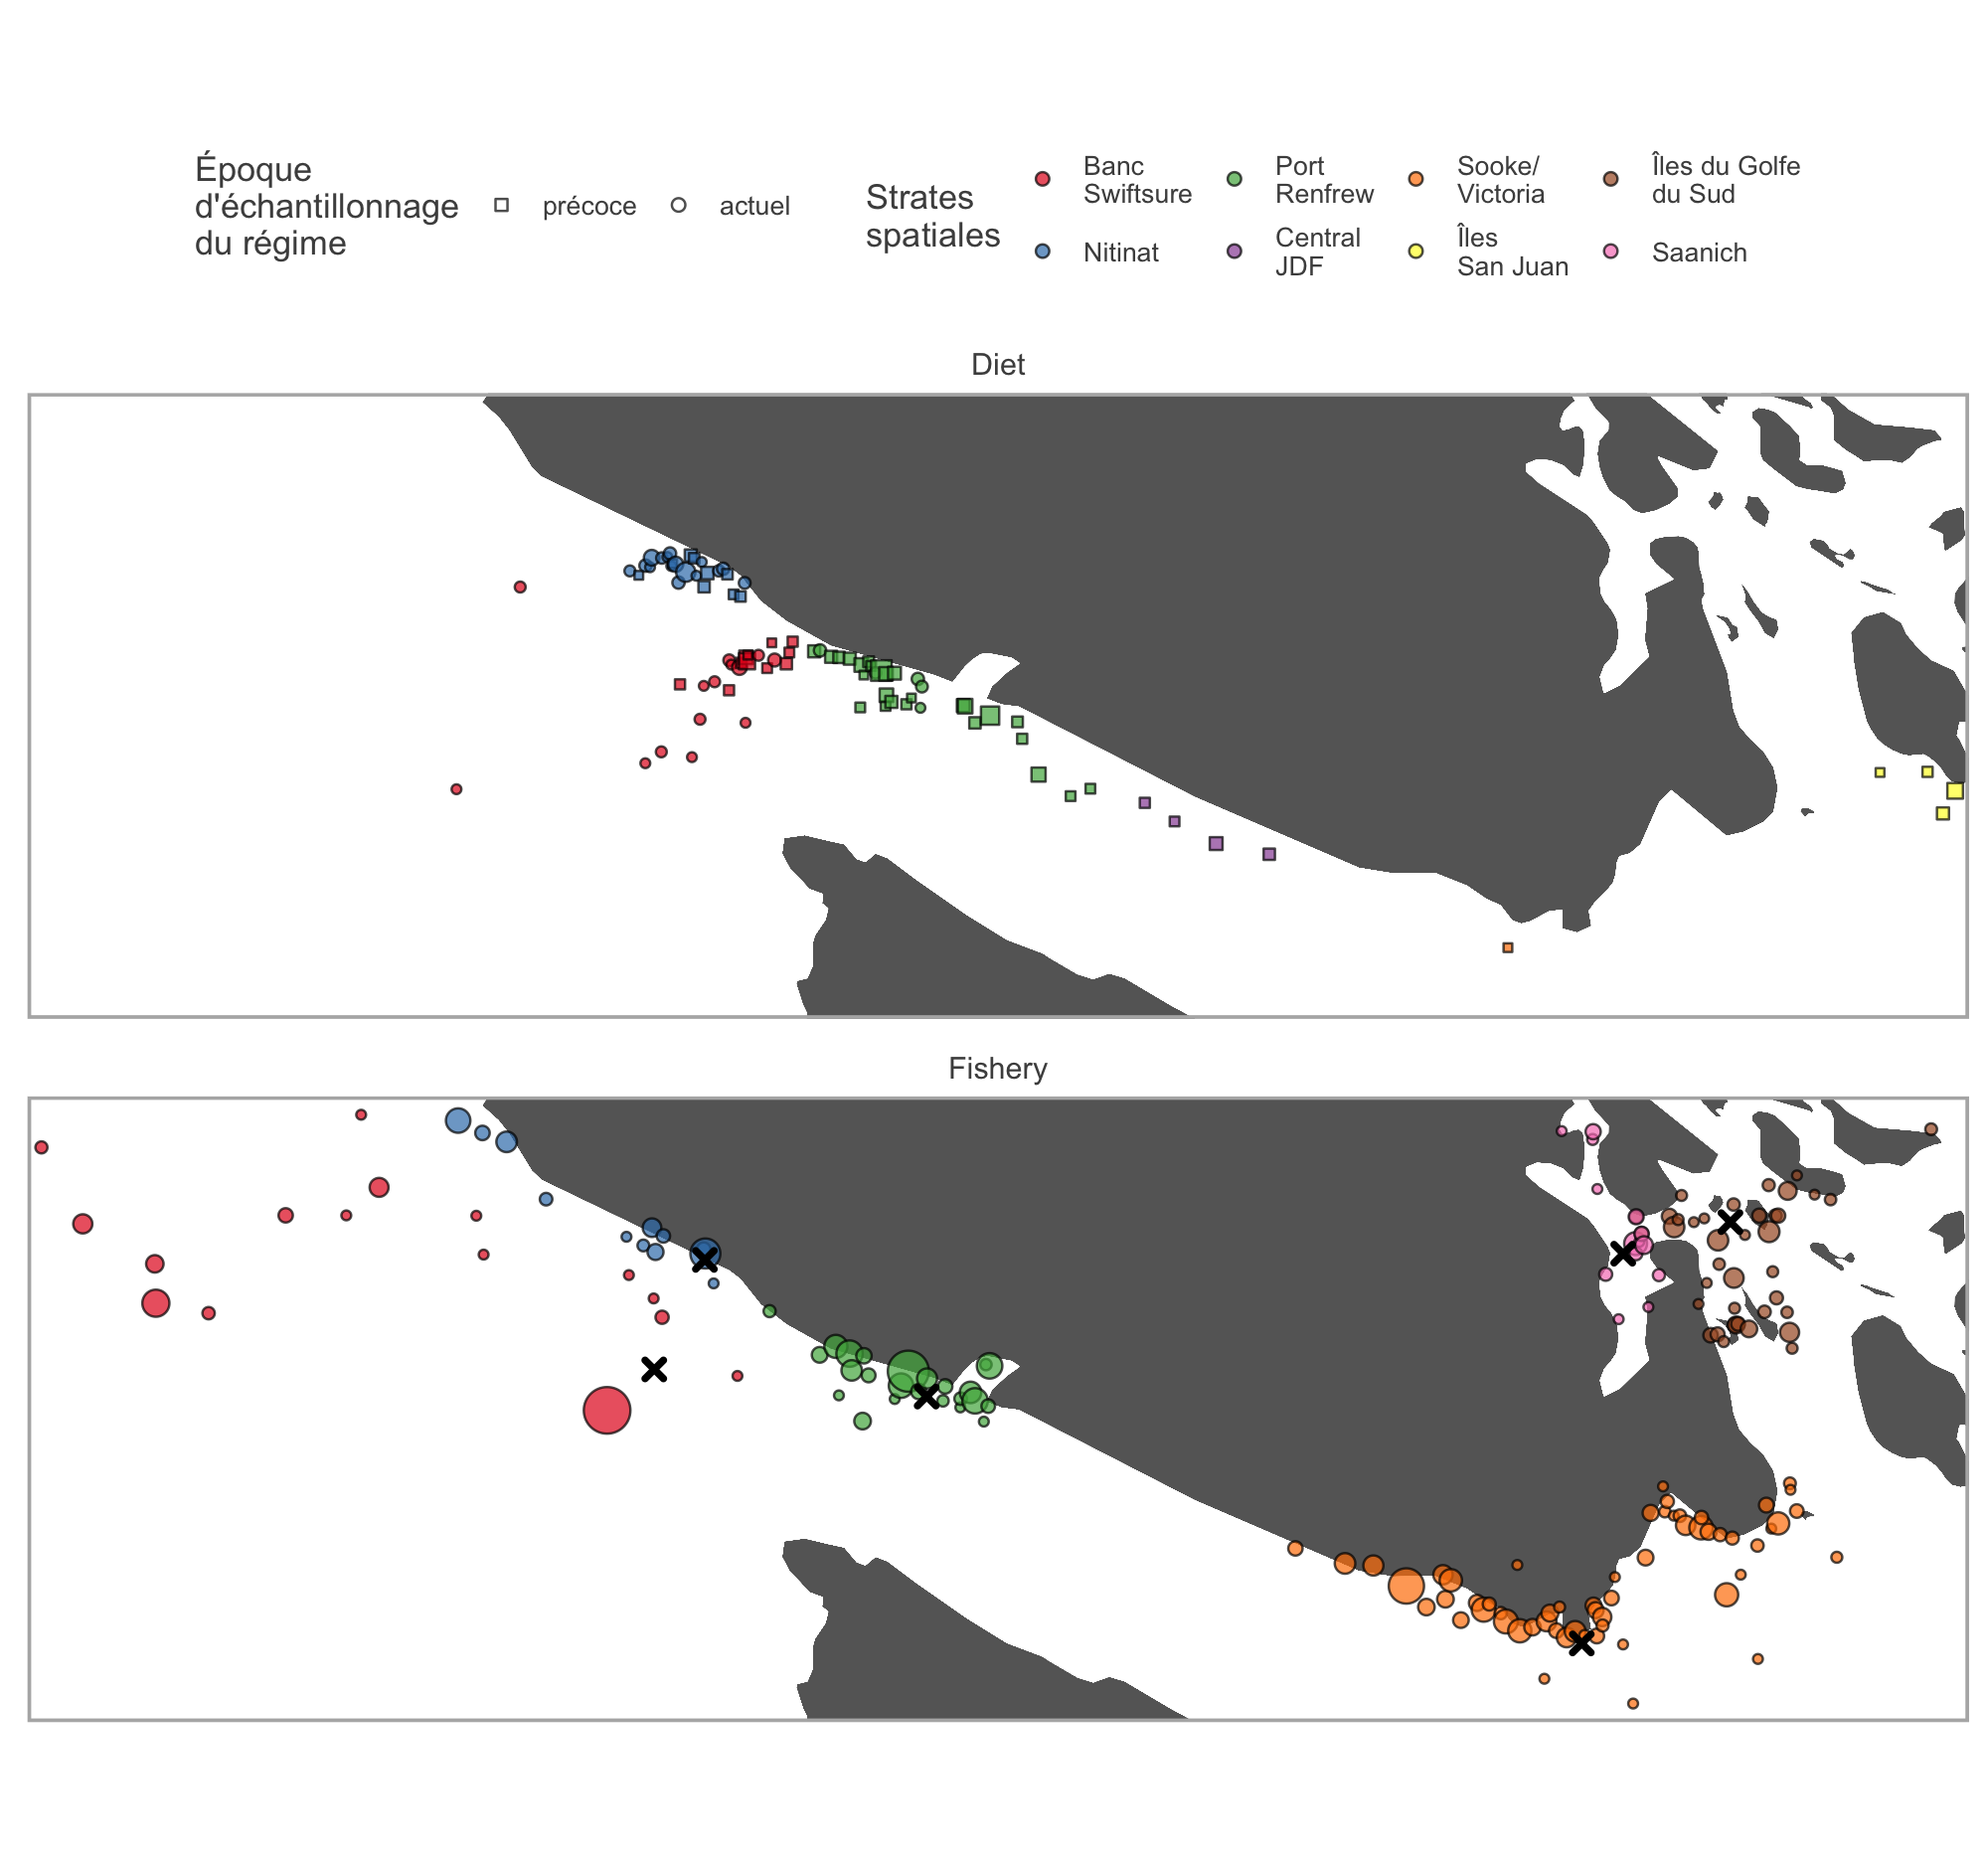
\includegraphics[width=5in]{figs/sampling_map.png}
    \caption{Emplacements des échantillons de composition des stocks de saumon chinook provenant des restes de proies de l'ÉRES (haut) et des pêcheries récréatives (bas). Les carrés et les cercles représentent les ères précoce (2003-2014) et actuelle (2017-2023), respectivement. Les points sont ombrés par strates spatiales et dimensionnés relativement au nombre d'échantillons collectés de cet emplacement sur toute la période d'étude. Les symboles 'x' noirs dans le panneau de pêcherie récréative sont des emplacements représentatifs dans chaque strate qui ont été utilisés pour générer des prédictions spatiales avec les modèles ajustés (Figures \ref{fig:stacked-rec}, \ref{fig:stacked-rec-size}). JDF central réfère au détroit de Juan de Fuca central.}
    \label{fig:sampling-map}
\end{figure}

Les protocoles de collecte d'échantillons utilisés dans les périodes d'échantillonnage précoce et actuelle étaient similaires. Quand des baleines étaient rencontrées, l'identification visuelle et photographique était initiée pour établir l'écotype, et si possible, déterminer le groupe, la matriligne, et/ou l'individu suivant les techniques d'identification décrites dans \cite{biggKillerWhalesStudy1987}. Le comportement des baleines était observé pour tout signe de comportement d'alimentation ou de fourrage actif (événements de prédation ; voir \citet{stredulinskyDelineatingImportantKiller2023} pour une description des indices comportementaux). Quand un événement de prédation est suspecté, le navire était déplacé à travers l'empreinte de nageoire caudale de la baleine pour chercher des écailles et tissus flottants. Les échantillons biologiques (p. ex., écailles, tissus de proie) étaient collectés en utilisant un filet à épuisette et retirés du filet en utilisant des pinces stériles et placés dans des fioles de scintillation en verre de 20 mL contenant 10 mL d'éthanol à 95\% pour identification subséquente. Les trois groupes d'ÉRES utilisent la partie ouest de l'habitat essentiel canadien pendant l'été et des restes de proies ont été collectés de chaque groupe, bien que trop peu étaient disponibles pour tester les différences spécifiques aux groupes.

Il est possible que les restes de proies échantillonnés puissent ne pas être représentatifs des régimes alimentaires de l'ÉRES. Premièrement, la diversité d'espèces dans les régimes alimentaires de l'ÉRES estimée à partir d'échantillons fécaux (présumés être non biaisés) est typiquement plus élevée que celle des échantillons de débris de proies \citep{hansonEndangeredPredatorsEndangered2021}, probablement due aux différences spécifiques aux espèces dans la probabilité que les débris soient collectés. Ces effets ne sont pas pertinents ici, cependant, parce que nous nous sommes concentrés seulement sur le saumon chinook. Deuxièmement, les restes de proies peuvent refléter les proies consommées près de la surface, qui peuvent être plus susceptibles d'être des proies orientées vers la surface ou de grande taille. Pourtant, les données de marquage suggèrent que les épaulards résidents identifient les proies de saumon du Pacifique à des profondeurs modérées, poursuivent des proies individuelles en eau profonde, et consomment ensuite les proies près de la surface \citep{wrightBehavioralContextEcholocation2021}. Ces comportements sont consistants à travers une gamme relativement large d'espèces et de classes de taille de saumon du Pacifique \citep{wrightBehavioralContextEcholocation2021}. Troisièmement, les événements d'échantillonnage de l'ÉRES peuvent ne pas être indépendants. Sans modèle statistique, nous ne pouvons pas quantifier l'autocorrélation spatiale ou temporelle dans les restes de proies ; cependant, les échantillons collectés le même jour et en proximité proche provenaient souvent de multiples stocks, suggérant une autocorrélation modeste (Figures \ref{fig:prey-samples-2007}, \ref{fig:prey-samples-2017}).

\begin{figure}[H]
    \pdftooltip{\centering
    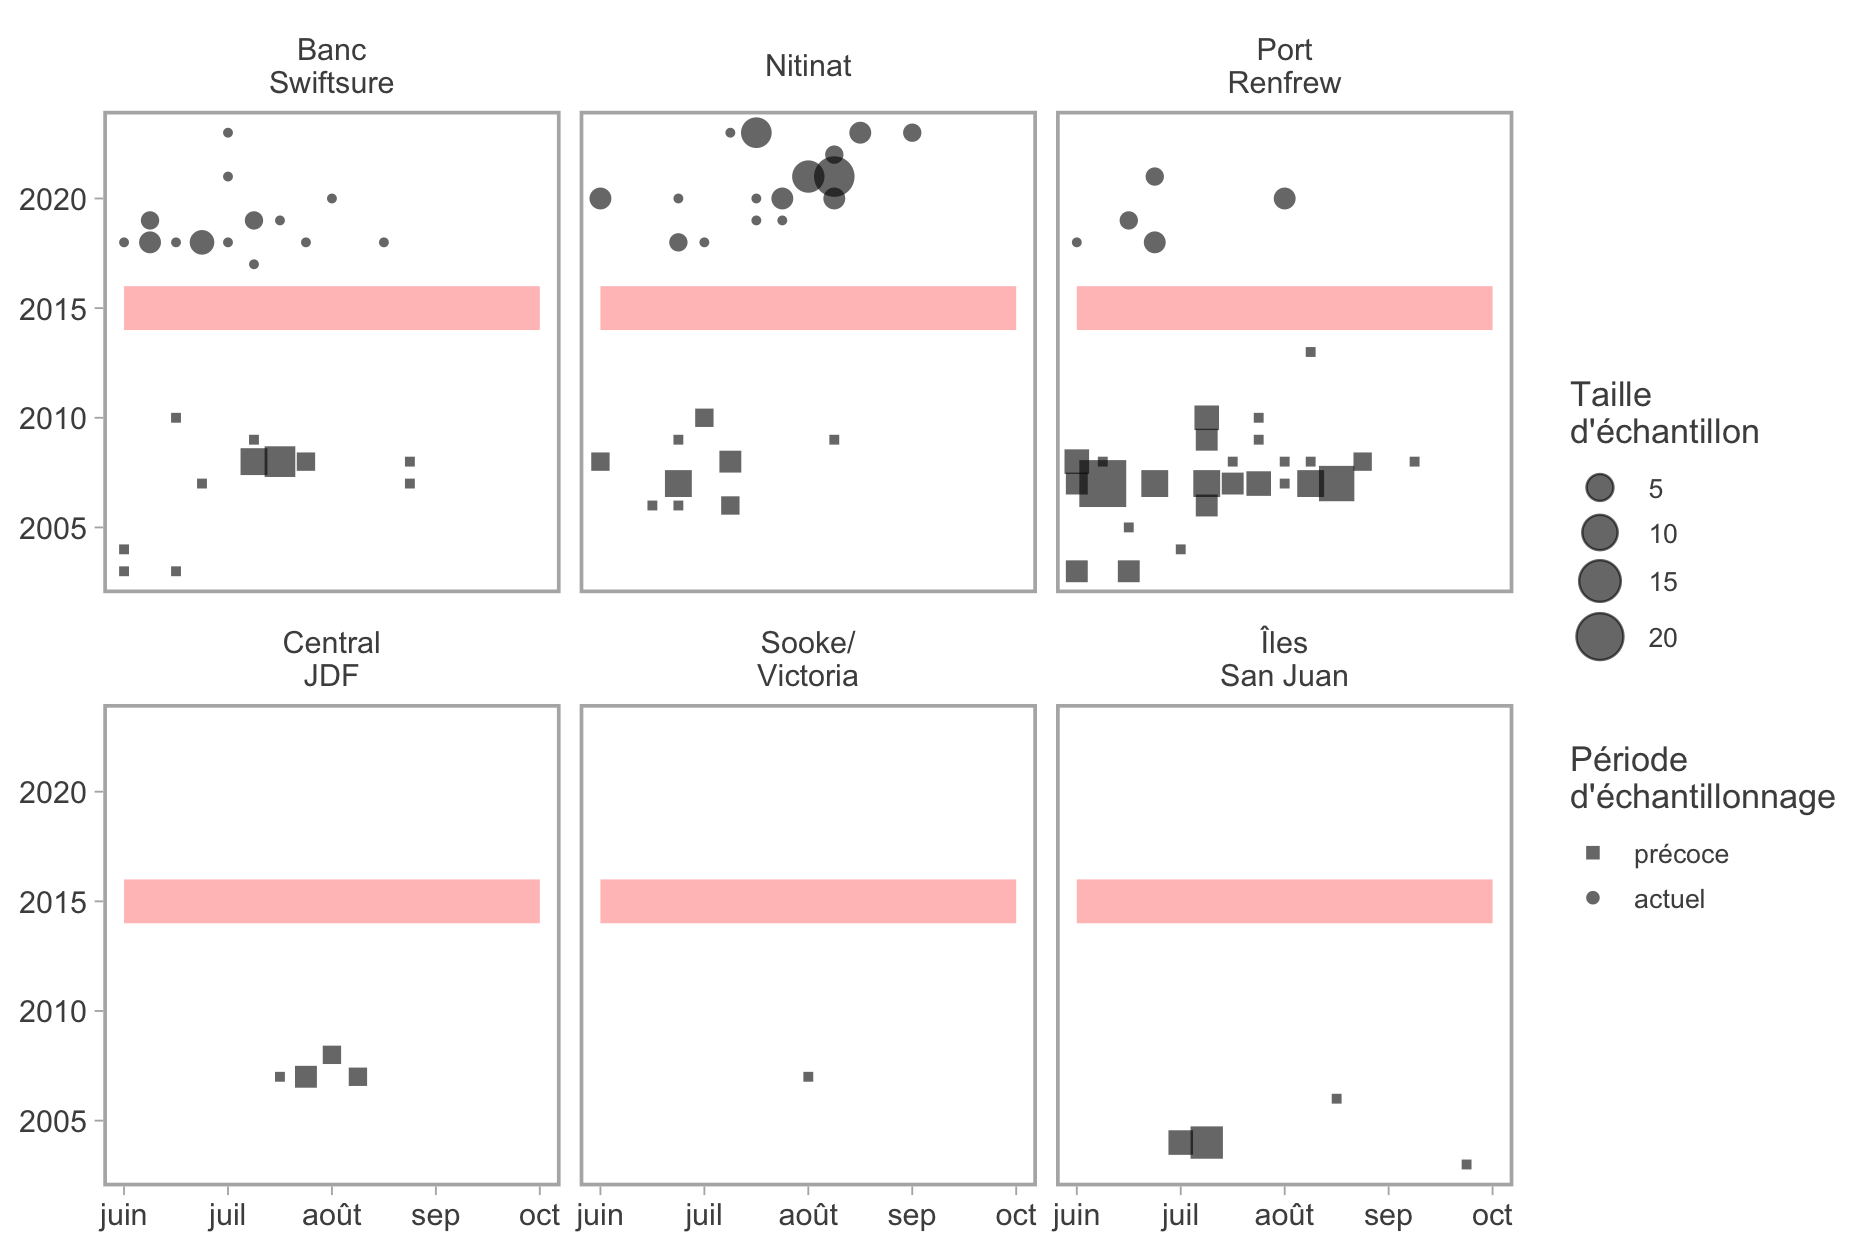
\includegraphics[width=5in]{figs/temporal_sample_coverage.png}}{Figure \ref{fig:temporal-diet-samples}}
    \caption{Distribution temporelle des échantillons de composition des stocks de saumon chinook des restes de proies de l'ÉRES. Les strates (panneaux) correspondent aux domaines spatiaux dans la Figure \ref{fig:sampling-map}. Les périodes d'échantillonnage précoce et actuelle sont représentées par des carrés et des cercles, respectivement, avec le polygone rouge montrant les années intermédiaires. La taille des points mise à l'échelle du nombre d'échantillons collectés dans une semaine et année données.}
    \label{fig:temporal-diet-samples}
\end{figure}

\subsection{Échantillonnage des pêcheries récréatives de saumon chinook}

La section d'évaluation des stocks de la côte sud du MPO collecte des données biologiques des pêcheries récréatives en eau salée à travers le sud de la Colombie-Britannique. Depuis 2014, ces données ont inclus des échantillons d'écailles et de tissus, des mesures de longueur à la fourche, de l'information sur si la nageoire adipeuse d'un poisson est intacte ou coupée, et, quand présentes, des marques à fil codé (MFC) qui assignent un individu à un groupe de lâcher d'écloserie spécifique. Des détails additionnels sur comment les échantillons biologiques sont utilisés pour déterminer l'âge et l'identité de stock sont fournis ci-dessous.

Les échantillons de pêcherie ont été collectés de trois programmes de terrain. La majorité provenait du programme d'observateur d'enquête au quai, où les échantillons sont collectés pendant des entrevues avec des pêcheurs récréatifs. Le programme d'observateur au quai échantillonne seulement les prises débarquées (c.-à-d., poissons retenus pour la récolte). Une portion d'échantillons a été collectée par un programme de science citoyenne, les Avid Anglers, qui est une collaboration entre le MPO, le British Columbia Sport Fishing Institute, les récolteurs récréatifs, et les guides de pêche sportive. Les participants fournissent des données sur la taille et le statut de coupe adipeuse pour tout le saumon qu'ils rencontrent (gardé et relâché), ainsi que des échantillons pour l'identification génétique de stock (IGS). Les échantillons proviennent principalement des prises débarquées ; cependant, les Avid Anglers collectent aussi des échantillons génétiques des poissons relâchés des pêcheries de non-rétention (bien que la fréquence d'échantillonnage dans les pêcheries de non-rétention varie spatialement). Finalement, les échantillons de 2022 et 2023 incluent des données collectées par le personnel scientifique du MPO pendant les Pêcheries de référence, un programme de recherche en collaboration avec le Sport Fishing Institute pour collecter des données biologiques pour évaluer les impacts des pêcheries sélectives de marque. Les Pêcheries de référence échantillonnent tout le saumon chinook rencontré et sont donc représentatives des prises débarquées et relâchées. Nous n'avons pas stratifié basé sur le programme de terrain parce que les échantillons Avid Angler des prises débarquées ne pouvaient pas être distingués de façon fiable de l'échantillonnage au quai des prises débarquées.

Les données dépendantes de la pêcherie peuvent être biaisées dues à des facteurs tels que la sélectivité de l'engin ou le comportement du pêcheur. Ces effets sont amplifiés par les interventions de gestion telles que les pêcheries sélectives de marque ou les limites de taille. Les pêcheries récréatives dans la zone d'étude ont été impactées par des interventions de gestion qui varient saisonnièrement, spatialement, et parmi les années (Figure \ref{fig:temporal-fishery-samples-management} ; voir Dobson et al. 2020 et MPO 2023 pour détails). Bien que notre ensemble de données inclut des échantillons d'individus relâchés, qui sont présumément moins biaisés que les prises débarquées, ceux-ci constituaient une proportion relativement petite du total (approximativement 5\%). Une analyse préliminaire a indiqué que les estimations de composition des stocks étaient similaires indépendamment de si les échantillons de poissons relâchés étaient ou n'étaient pas inclus (résultats non montrés), et toutes les analyses subséquentes ont inclus les échantillons relâchés. Malheureusement, une évaluation plus robuste des effets de sélectivité n'était pas possible due au calendrier et à l'emplacement déséquilibrés des mesures de gestion ; cependant, nous décrivons qualitativement les impacts potentiels des mesures de gestion à nos conclusions dans la discussion.

Les échantillons biologiques incluaient un code d'emplacement représentant l'emplacement de pêche (soit rapporté à l'observateur d'enquête ou enregistré par l'Avid Angler ou le personnel scientifique). Les codes d'emplacement étaient géoréférencés pour fournir une latitude et longitude pour chaque échantillon. En d'autres mots, chaque échantillon de pêcherie avait un emplacement approximatif représentant un site de pêche communément utilisé, pas un emplacement précis basé sur où le poisson a été capturé (Figure \ref{fig:sampling-map}). Bien que la couverture variait spatialement, l'échantillonnage a eu lieu dans certaines régions dans tous les mois (Figure \ref{fig:temporal-fishery-samples}).

\begin{figure}[H]
    \centering
    \pdftooltip{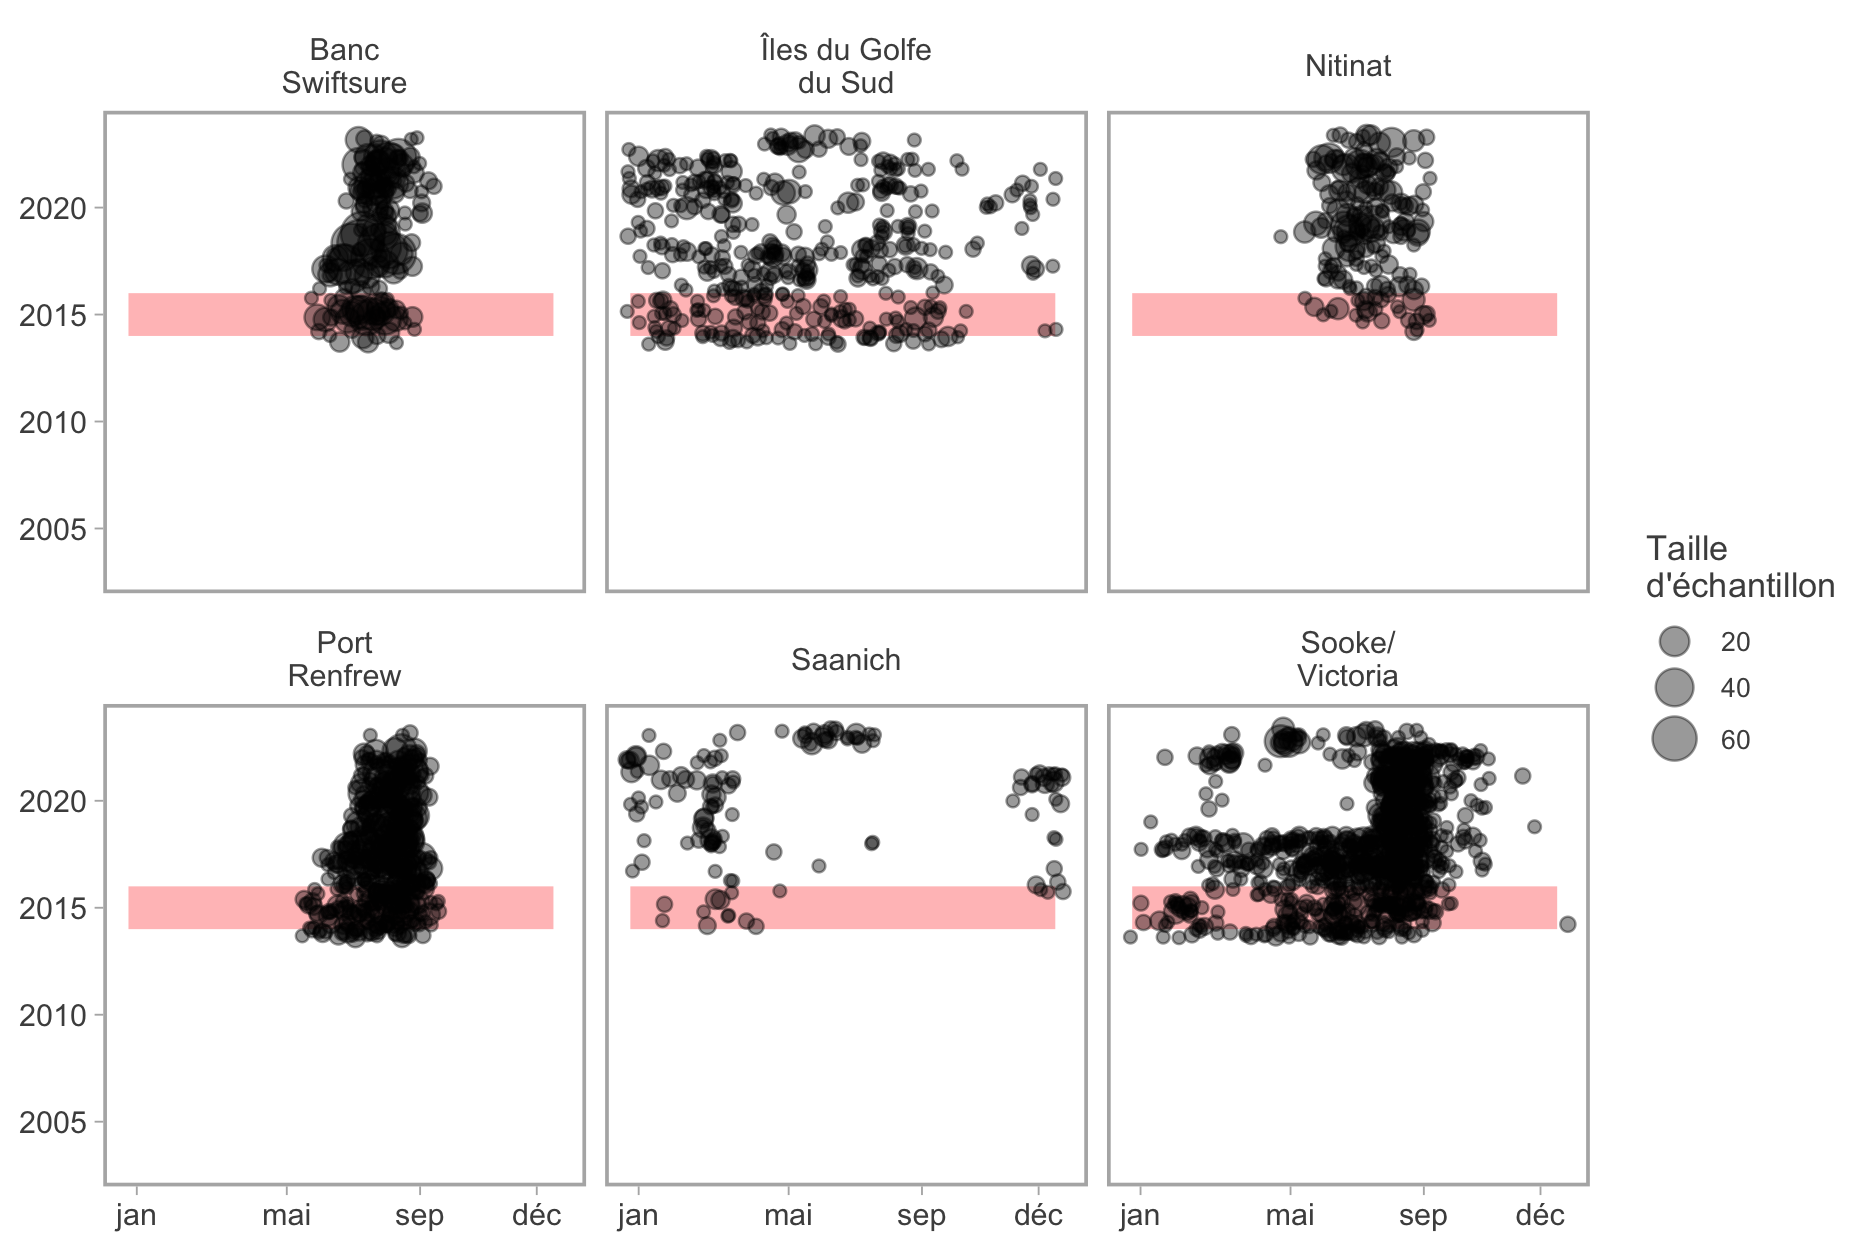
\includegraphics[width=5in]{figs/rec_temporal_sample_coverage.png}}{Figure \ref{fig:temporal-fishery-samples}}
    \caption{Distribution temporelle des échantillons de composition des stocks de saumon chinook des pêcheries récréatives. Les strates (panneaux) correspondent aux domaines spatiaux dans la Figure \ref{fig:sampling-map}. Les années intermédiaires sans échantillons de proies sont représentées par un polygone rouge montrant qu'aucun échantillon de pêcherie n'est disponible de la période d'échantillonnage précoce des restes de proies de l'ÉRES (Figure \ref{fig:temporal-diet-samples}). La taille des points mise à l'échelle du nombre d'échantillons individuels collectés dans un emplacement de pêche, une semaine, et une année donnés. Les points ont été décalés pour maximiser la visibilité. Notez que les échantillons de pêcherie, contrairement aux échantillons de restes de proies, ont été collectés tout au long de l'année.}
    \label{fig:temporal-fishery-samples}
\end{figure>

L'avantage principal de cet ensemble de données relativement aux données de récupération de MFC plus communément utilisées est la précision avec laquelle les échantillons peuvent être assignés à un emplacement et une période de temps. Le programme MFC vise à estimer les taux d'exploitation spécifiques aux stocks à travers une échelle spatiale large — un objectif similaire, mais distinct, à l'estimation des estimations spatialement et temporellement explicites de composition des stocks. Parce que les estimations dérivées de MFC des taux d'exploitation requièrent un nombre relativement grand de récupérations de marques par pêcherie pour être suffisamment précises, elles sont communément agrégées à des échelles saisonnières (p. ex., multiples mois) et régionales (p. ex., sud-ouest de l'île de Vancouver vs. sud du détroit de Georgie). De plus, plusieurs stocks canadiens, incluant Fraser River Spring $5_2$ et Summer $5_2$, qui peuvent être des proies clés des ÉRES ne sont pas adéquatement représentés par les indicateurs MFC actuels.

\subsection{Assignation des échantillons aux stocks, classes de taille, et écloseries}

\subsubsection{Échantillons de proies de l'ÉRES}

Les écailles collectées après un événement de prédation de l'ÉRES ont été montées et examinées visuellement en utilisant des projecteurs Leitz Neopromar pour évaluer les patrons d'anneaux marins et d'eau douce. L'espèce et l'âge ont été déterminés des lectures d'écailles par des âgeurs expérimentés au Laboratoire de vieillissement des poissons au Laboratoire de sclérochronologie de la Station biologique du Pacifique (Pêches et Océans Canada, Nanaimo, Colombie-Britannique, Canada). Le laboratoire fournit une estimation du nombre d'années qu'un saumon a passé dans les habitats d'eau douce et océanique (c.-à-d., âge d'eau douce et marin respectivement) basée sur les incréments de croissance annuels. Puisque la majorité de la croissance du saumon chinook se produit pendant la résidence océanique et les âges d'eau douce n'étaient pas toujours disponibles pour les échantillons de pêcherie, nous avons concentré les analyses sur l'âge marin. De plus, nous avons incorporé l'erreur de vieillissement dans les estimations des restes de proies de l'ÉRES et utilisé l'âge marin, incluant cette erreur, pour prédire la longueur à la fourche des proies de l'ÉRES basée sur les relations taille-selon-l'âge spécifiques aux stocks (détails dans l'Appendice \ref{size-at-age}).

Les échantillons d'écailles et les restes de tissus post-prédation ont été soumis au Laboratoire de génétique moléculaire du MPO à la Station biologique du Pacifique pour l'identification d'espèce et de stock. L'identification des stocks de saumon chinook a suivi la méthodologie décrite dans Beacham et al. (2018)\nocite{beachamParentagebasedTaggingGenetic2022}. Brièvement, l'ADN a été extrait et l'amplification PCR de 321 amplicons cibles a été conduite en utilisant un pool d'amorces développé à partir de données de séquence de saumon chinook publiées. Les échantillons ont ensuite été identifiés au stock en utilisant soit a) une méthodologie de séquençage d'amplicon SNP ciblée ou b) des marques basées sur la parenté (PBT). Sous le programme PBT, les géniteurs d'écloserie sont génotypés, permettant aux descendants échantillonnés d'être assignés aux individus parents et identifiés comme d'origine d'écloserie (détails ci-dessous), avec un haut degré de confiance \citep{beachamParentagebasedTaggingGenetic2022}. Nous avons agrégé les assignations de stocks individuels pour améliorer l'interprétabilité (détails additionnels ci-dessous).

\subsubsection{Échantillons de pêcherie récréative}

L'identité de stock pour les échantillons collectés de la pêcherie récréative a été inférée en faisant correspondre les MFC ou otolithes récupérés aux cohortes de lâcher ou en utilisant des échantillons de tissus avec des SNP ou des microsatellites \citep{beachamPacificRimPopulation2006a, beachamParentagebasedTaggingGenetic2022}. Étant donné le grand nombre de stocks de saumon chinook présents dans le sud de la Colombie-Britannique, nous avons agrégé les assignations individuelles, qui ont été faites approximativement à l'échelle des populations de frai, pour rendre les analyses subséquentes traitables.

Au Canada, le saumon chinook est évalué au niveau de l'UC \citep{holtbyConservationUnitsPacific2007} ; cependant, les actions de gestion domestiques se concentrent souvent sur les unités de gestion de stock (UGS) qui contiennent une ou plusieurs UC. Bien que les UC dans une UGS peuvent ne pas frayer en proximité proche, une seule UGS a typiquement une distribution marine et une phénologie de migration relativement homogènes. Les UC par définition excluent les poissons d'origine d'écloserie, tandis que les UGS ne le font pas. Puisque notre analyse était concentrée sur le contexte de gestion canadien, nous avons agrégé la plupart des populations canadiennes au niveau UGS (Figure \ref{fig:stock-map}, Tableau S1). Nous avons de plus agrégé les UGS Lower Georgia Strait, Middle Georgia Strait, Upper Georgia Strait, et Southern Mainland Inlet comme East Coast Vancouver Island et Southern Mainland Inlets (ECVI/SOMN) puisque ces UGS étaient relativement rarement rencontrées (Figure \ref{fig:stock-map}, Tableau S1). Nous avons assigné les individus restants à un de quatre groupements régionaux : Puget Sound, Columbia River et Snake River spring-run, Columbia et Snake river summer/fall-run (incluant les poissons Willamette River spring-run due à une distribution marine similaire), et un agrégat (« Autre ») incluant les populations rares du nord de la Colombie-Britannique, de la côte de Washington et Oregon, et de Californie (Figure \ref{fig:stock-map}, Tableau S1). Nous soulignons que les stocks Columbia River et « Autre » regroupent des populations avec des histoires de vie disparates, mais étant donné le focus de gestion canadien de cette analyse et la nécessité d'ajuster un modèle traitable, nos groupements permettent qu'une inférence raisonnable soit tirée. À travers ce manuscrit, nous utilisons les termes « stock » et « composition des stocks » quand nous référons à ces groupements spécifiques, ainsi qu'aux agrégats génériques de populations de saumon chinook.

\begin{figure}[H]
    \centering
    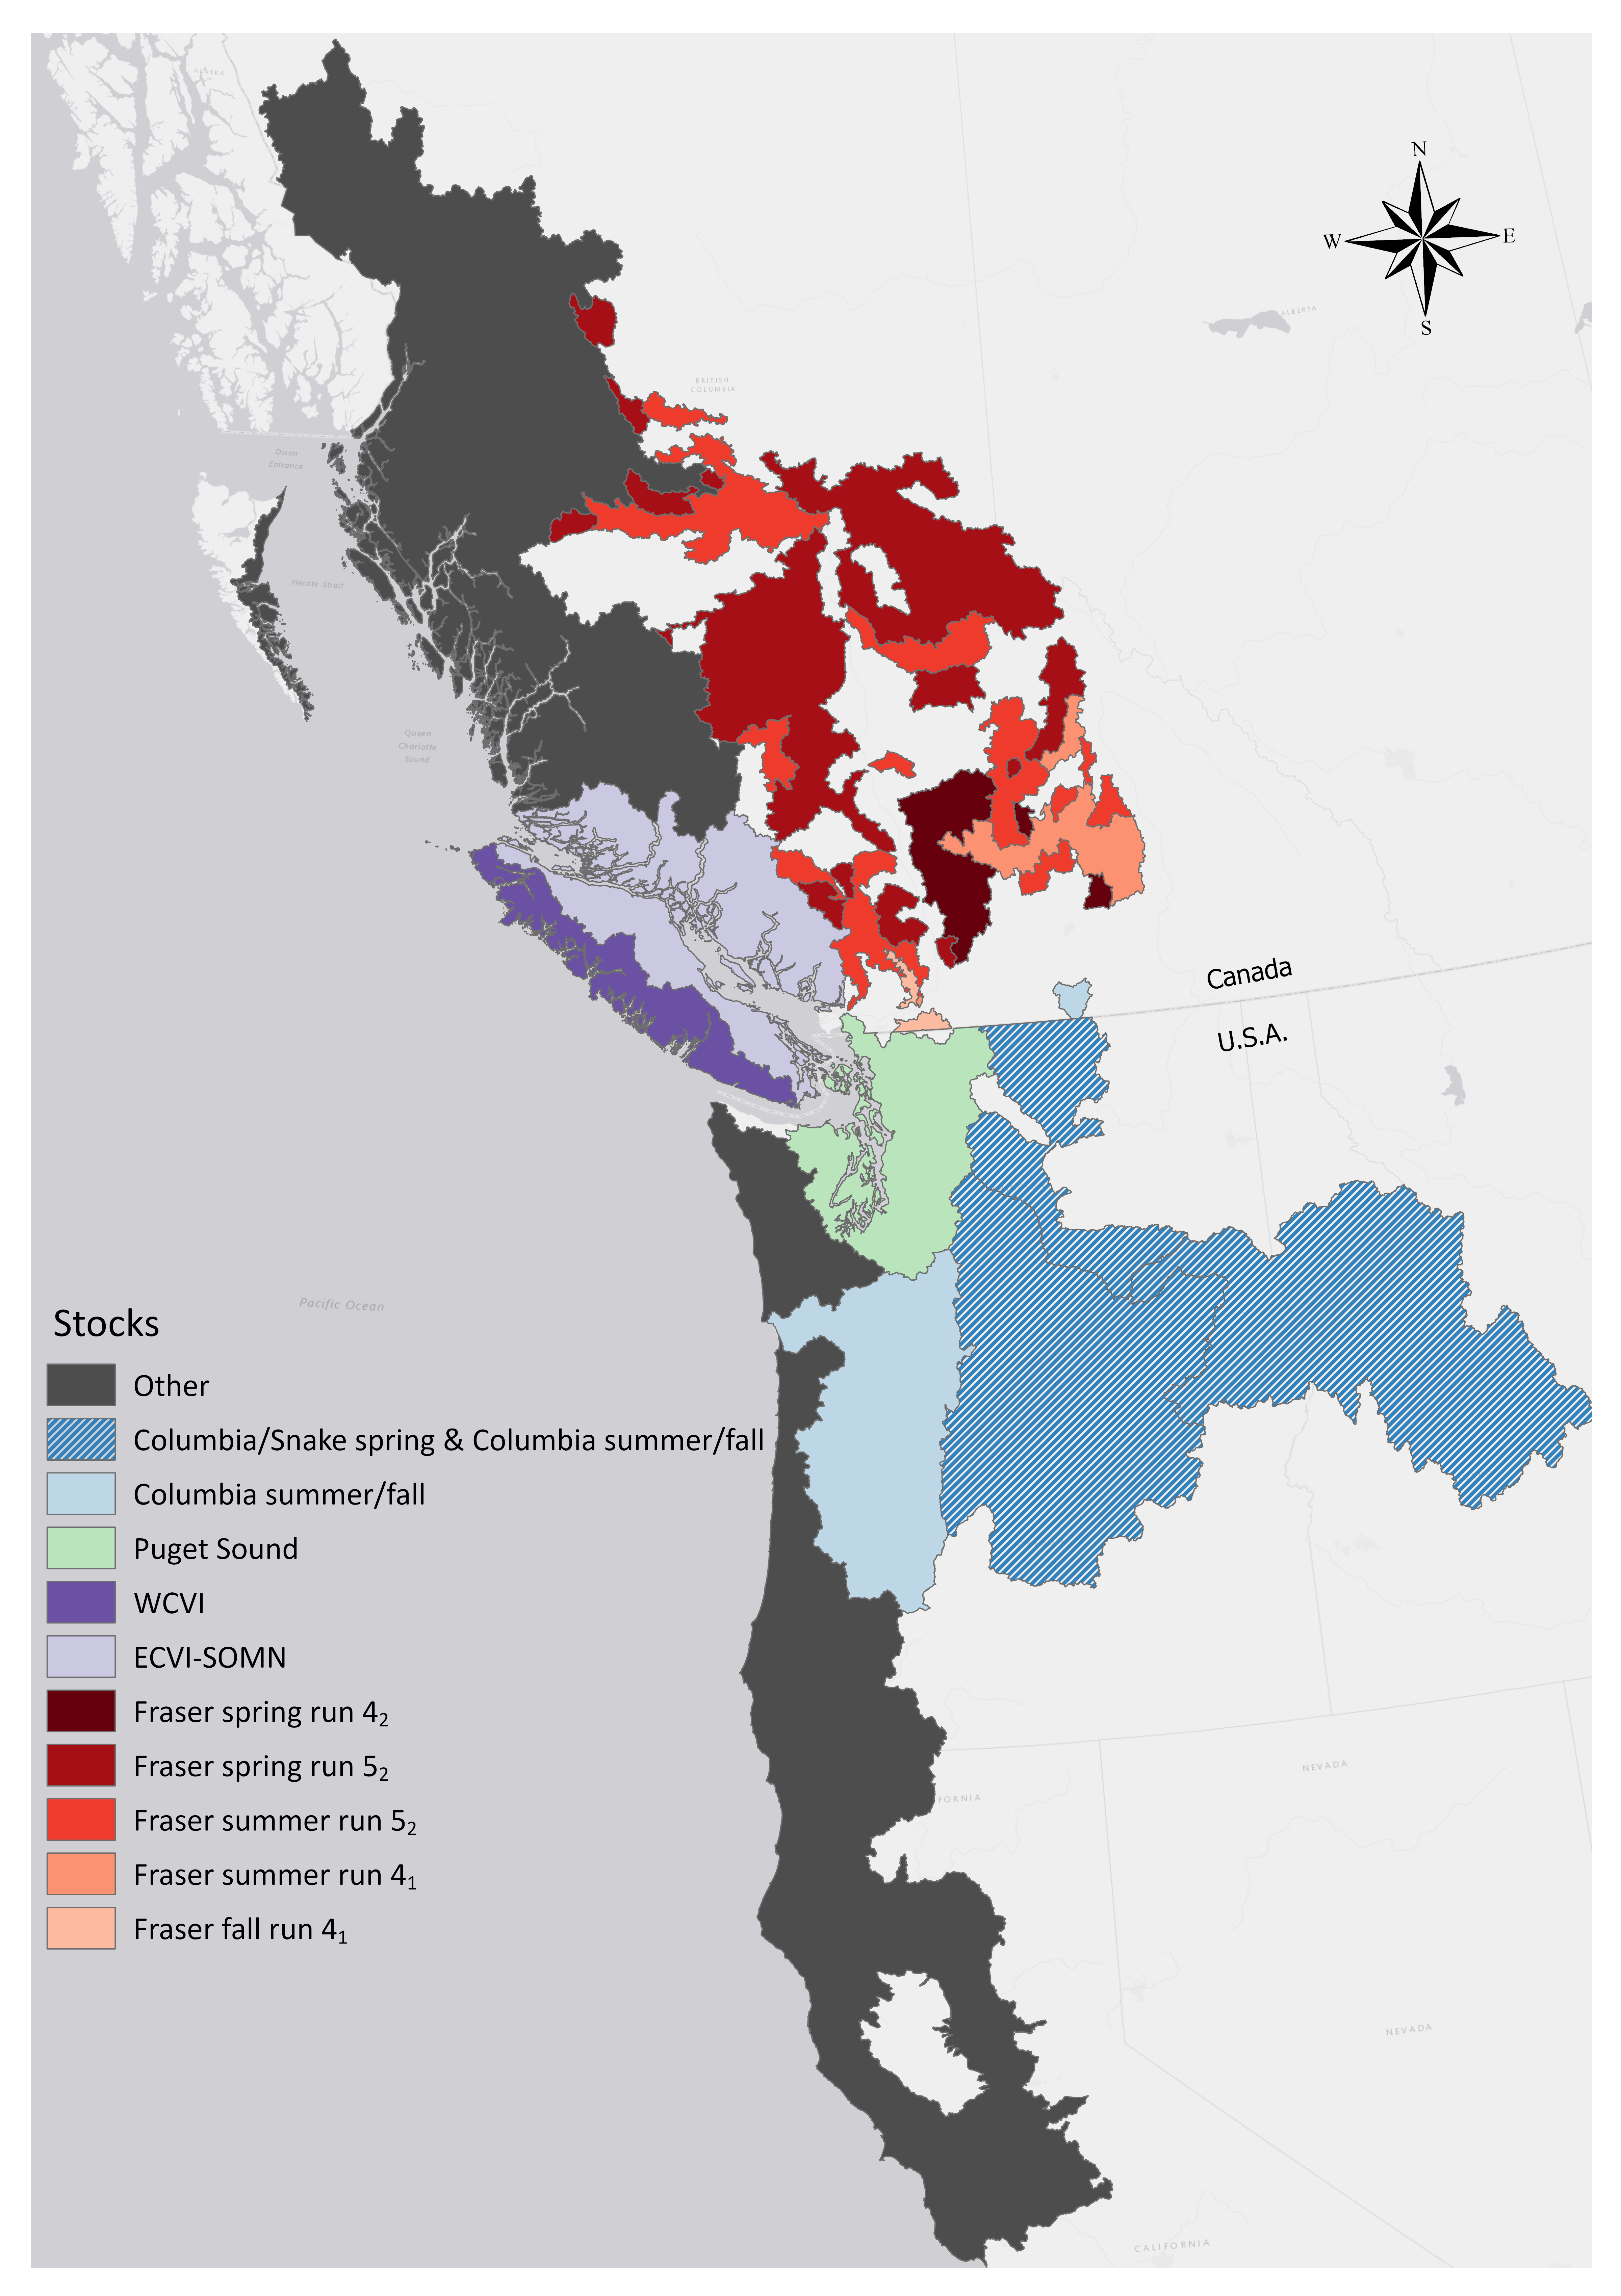
\includegraphics[width=5in]{figs/chinook_stock_map.png}
    \caption{Bassins versants contenant les cours d'eau natals pour chaque stock de saumon chinook. Notez que tous les bassins versants avec des populations Columbia River Spring contenaient aussi des populations Columbia River Summer/Fall et sont représentés par des hachures.}
    \label{fig:stock-map}
\end{figure}

Pour modéliser la variabilité dans la taille du saumon chinook, nous avons créé quatre casiers de taille basés sur la longueur à la fourche à la capture : moins de 65 cm, 65-75 cm, 75-85 cm, et plus de 85 cm. Les poissons plus petits que les limites de taille minimales (soit 62 ou 45 cm de longueur à la fourche selon la zone de gestion) peuvent être échantillonnés et relâchés ; cependant, nous avons inclus seulement les poissons plus grands que 55 cm dans les analyses subséquentes. Les données d'âge pour un sous-ensemble d'individus (n = 7815) étaient disponibles des MFC, PBT, ou estimées en utilisant les anneaux d'écailles (détails ci-dessus).

Nous avons utilisé de multiples approches pour identifier la contribution relative des poissons d'origine d'écloserie dans les échantillons des pêcheries récréatives. Les poissons avec des nageoires adipeuses manquantes ont été identifiés comme d'origine d'écloserie. Les taux de marquage (la proportion de lâchers d'écloserie où les nageoires adipeuses sont retirées) sont presque 100\% dans les écloseries de Washington et Oregon \citep{andersonReviewHatcheryReform2020, wdfwAnadromousSalmonSteelhead2021, odfwFishPropagationAnnual2022}, mais les écloseries de Colombie-Britannique marquent seulement une proportion relativement petite d'individus \citep{pscLessonsLearnedReport2016}. Par conséquent, nous avons aussi utilisé les marques thermiques d'otolithes et l'échantillonnage génétique pour identifier les individus d'origine d'écloserie.

Les écloseries de Colombie-Britannique ont commencé à implémenter le PBT dans l'année de géniteur 2013 et bien que la couverture dans les grandes installations d'amélioration soit typiquement élevée, elle a varié dans le temps (Figure \ref{fig:pbt-coverage}). Les individus avec une assignation PBT ont été identifiés comme d'origine d'écloserie, tandis que ceux identifiés comme provenant de stocks qui ne sont pas présents dans la ligne de base PBT ont été identifiés comme sauvages. Finalement, les individus avec des nageoires adipeuses intactes et des assignations GSI à des stocks avec de faibles taux de marquage et aucune donnée PBT (p. ex., Californie, Alaska) ou appartenant à des années de géniteur dans lesquelles l'écloserie pertinente de Colombie-Britannique avait un taux PBT relativement faible (ici défini comme moins de 80\% de couverture de géniteurs (Figure \ref{fig:pbt-coverage})) ont été assignés une classification « inconnue ». Étant donné que de nombreux échantillons de pêcherie récréative ne pouvaient pas être assignés de façon définitive un statut d'écloserie ou sauvage, et que les contributions d'écloserie covarient avec l'identité de stock, nous n'avons pas ajusté un modèle statistique aux données assignées d'écloserie.

Contrairement aux analyses précédentes \cite[p. ex.,][]{freshwaterIntegratedModelSeasonal2021}, nous n'avons pas mis à l'échelle les estimations de composition des stocks par les prises de saumon chinook par unité d'effort pour dériver un indice d'abondance spécifique aux stocks parce que la comparaison principale d'intérêt était entre la composition de la pêcherie et la composition des restes de proies. De plus, les estimations de prises et d'effort sont typiquement les plus fiables aux échelles de sous-zone d'enquête et mensuelles (ou plus grossières), ce qui diluerait la résolution spatio-temporelle des estimations de composition des stocks. Finalement, nous assumons déjà que la pêcherie récréative échantillonne la composition du saumon chinook d'une manière analogue aux ÉRES (exploré en détail dans la Discussion). Les estimations d'abondance spécifiques aux stocks incorporent des assumptions de sélectivité additionnelles qui peuvent ne pas être valides.

\subsection{Proportion de géniteurs d'origine d'écloserie}

Pour mieux comprendre la variation parmi les stocks canadiens dans l'amélioration d'écloserie, nous présentons à la fois des estimations basées sur l'individu des contributions d'écloserie (décrites dans la section précédente) et des estimations de la proportion de géniteurs d'origine d'écloserie (pHOS). Les estimations de pHOS ont été fournies par le Programme d'amélioration des salmonidés de Pêches et Océans Canada et étaient disponibles pour les années de retour entre 2014 et 2022, bien que le nombre d'années disponibles variait parmi les populations de frai. Puisque chaque stock contient de multiples populations de frai, nous avons calculé le pHOS moyen, par stock, en utilisant un modèle hiérarchique avec des ordonnées à l'origine aléatoires pour la population et un lien bêta. Les estimations de pHOS moyen au niveau de stock devraient être interprétées avec caution puisque relativement peu de populations par stock ont été considérées et les moyennes ne sont pas pondérées par l'abondance relative de chaque population. De plus, pHOS ne fournit pas un indice de l'abondance \textit{globale} des poissons d'écloserie dans un stock, seulement un indice de l'abondance d'écloserie sur les frayères.

\subsection{Abondance terminale du saumon chinook}

Les tendances récentes de l'abondance du saumon chinook ont été rapportées ailleurs \cite[p. ex.,][]{atlasTrendsChinookSalmon2023, ctcAnnualReportCatch2024a} ; cependant, pour contexte additionnel, nous présentons des estimations d'abondance terminale groupées par les stocks focaux dans notre analyse. Les estimations d'abondance terminale incluent l'échappée ainsi que la récolte dans les zones terminales, à l'exception des estimations ECVI/SOMN qui incluent seulement l'échappée. Les zones terminales sont généralement définies comme l'eau douce, mais les estimations de certains stocks incluent aussi la récolte dans les pêcheries marines proximales à l'eau douce (Tableau \ref{tab:sources}). Nous présentons les données d'abondance terminale de 1982 à 2023, mais des moyennes de quatre ans ont été utilisées pour interpoler les valeurs 2023 pour la plupart des stocks Washington Coastal (groupés avec Autre à travers ce manuscrit) et Puget Sound. Détails additionnels dans l'Appendice \ref{terminal-abundance}.

Les estimations d'abondance terminale fournissent un indice d'abondance dans l'habitat essentiel de l'ÉRES canadien, mais seront biaisées relativement à la vraie abondance parce qu'elles excluent la récolte dans les pêcheries marines et la mortalité naturelle. De plus, les estimations d'abondance terminale échouent à tenir compte des différences spécifiques aux stocks dans le calendrier de remontée, les routes de migration, et, dans le cas des stocks de saumon chinook résidents, les individus immatures qui croissent dans l'habitat essentiel de l'ÉRES pour des périodes étendues. Ces facteurs impacteront l'abondance des proies disponible pour l'ÉRES ; cependant, tenir compte de leurs effets était à l'extérieur de la portée de l'analyse actuelle (détails additionnels décrits dans la Discussion).